\documentclass[tikz,border=8pt]{standalone}
% Shared look for every TikZ diagram. Load with \input{../../tools/tikz-style.tex}
\usepackage[T1]{fontenc}
\usepackage{lmodern}
\renewcommand{\sfdefault}{lmr}  % diagrams use the same serif as the text
\usetikzlibrary{arrows.meta, positioning, shapes.geometric, calc, fit, backgrounds}
\definecolor{cblue}{HTML}{4C78A8}
\definecolor{corange}{HTML}{F58518}
\definecolor{cgreen}{HTML}{54A24B}
\definecolor{cred}{HTML}{E45756}
\definecolor{cpurple}{HTML}{B279A2}
\definecolor{cgrey}{HTML}{6B6B6B}
\tikzset{
  every picture/.style={font=\sffamily, line width=1.2pt},
  box/.style={draw=#1, fill=#1!12, rounded corners=4pt, align=center, inner sep=7pt, minimum height=1.1cm},
  box/.default=cgrey,
  arrow/.style={-{Stealth[length=3mm]}, draw=cgrey, line width=1.4pt},
  title/.style={font=\sffamily\bfseries\Large},
  note/.style={font=\sffamily\small, text=cgrey, align=center},
}
\AtBeginDocument{\hyphenpenalty=10000 \exhyphenpenalty=10000}

\begin{document}
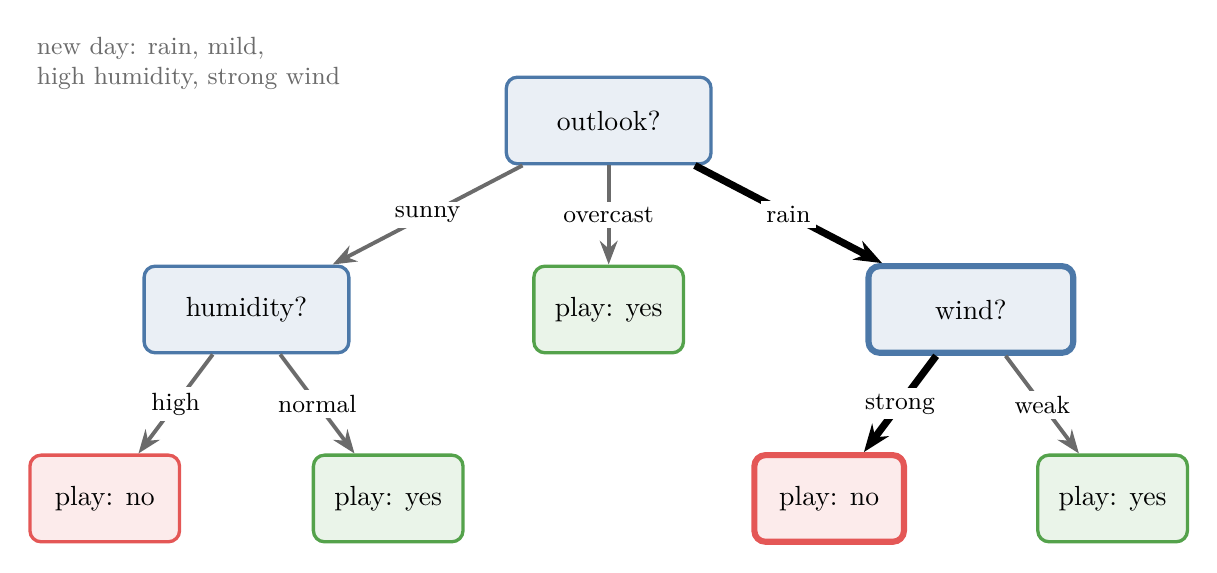
\begin{tikzpicture}[
  q/.style={box=cblue, minimum width=2.6cm},
  yes/.style={box=cgreen, minimum width=1.9cm},
  no/.style={box=cred, minimum width=1.9cm},
  lab/.style={font=\sffamily\small, fill=white, inner sep=2pt},
  path/.style={-{Stealth[length=3.5mm]}, draw=black, line width=2.6pt}]
  \node[q] (o) at (0,0) {outlook?};
  \node[q] (h) at (-4.6,-2.4) {humidity?};
  \node[yes] (ov) at (0,-2.4) {play: yes};
  \node[q, line width=2.2pt] (w) at (4.6,-2.4) {wind?};
  \node[no] (hh) at (-6.4,-4.8) {play: no};
  \node[yes] (hn) at (-2.8,-4.8) {play: yes};
  \node[no, line width=2.2pt] (ws) at (2.8,-4.8) {play: no};
  \node[yes] (ww) at (6.4,-4.8) {play: yes};
  \draw[arrow] (o) -- node[lab] {sunny} (h);
  \draw[arrow] (o) -- node[lab] {overcast} (ov);
  \draw[path] (o) -- node[lab] {rain} (w);
  \draw[arrow] (h) -- node[lab] {high} (hh);
  \draw[arrow] (h) -- node[lab] {normal} (hn);
  \draw[path] (w) -- node[lab] {strong} (ws);
  \draw[arrow] (w) -- node[lab] {weak} (ww);
  \node[note, align=left, anchor=north west] at (-7.4,1.2) {new day: rain, mild,\\high humidity, strong wind};
\end{tikzpicture}
\end{document}
